\chapter{Reverse Enginering}\label{chapter:reverse_engineering}

In this chapter we will present the results obtained and the observations made while reverse engineering the code of the Bank System application.
We will focus on the Smart Card Simulator Java application as well as the C batch transaction parser in order to analyze potential vulnerabilities, reverse engineer the TAN generation algorithm and ultimately make a direct comparison with the Goliath National Bank application.

\section{Smart Card Simulator}
The SCS application provided by Bank System requires the user to input his PIN, then allows to either insert the details (destination account, amount) for a single transaction or load a batch file for a multiple transaction.\newline
After having decompiled the code using the JavaDecompiler tool, we run the FindBugs plugin for IntelliJ IDEA on the source code of both the Bank System application and the GNB application.\newline

\subsection{FindBugs}
The Bank System static code analysis didn't return any specific vulnerabilities, as visible in \ref{figure:bs_findBugs}.\newline
One performance issue arised because of String concatenation inside a loop, which isn't really significative. There were also some dodgy code warnings regarding the usage of uninitialized variables (graphical components), which are irrelevant for this specific case, since Bank System uses a JavaFX application that binds the variables automatically thanks to the .fxml files. The warnings regarding unwritten variables are also uninmportant, for the same reason.

\begin{figure}[h!tbp]
	\centering
	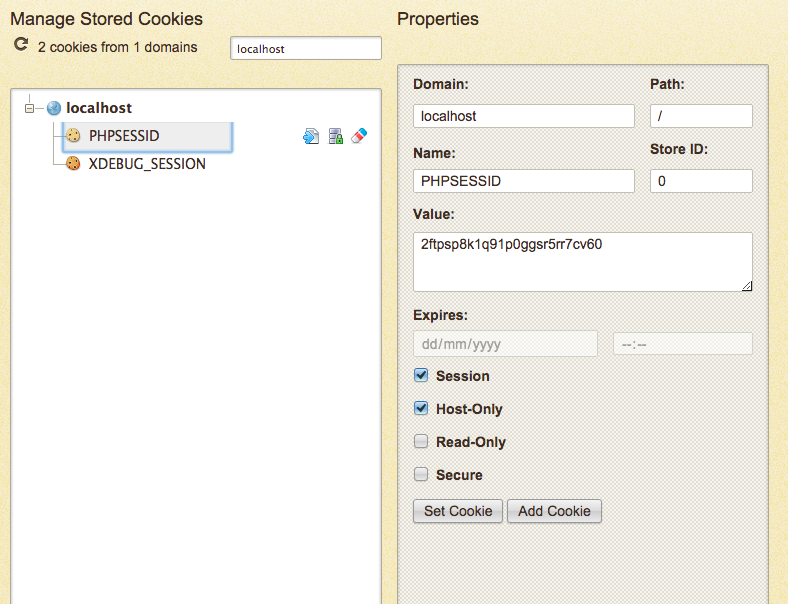
\includegraphics[width=\textwidth]{figures/bs_findBugs}
	\caption{Analysis results for Bank System}
	\label{figure:bs_findBugs}
\end{figure}

The static code analysis of the Goliath National Bank application on the other hand returned significantly more issues, most of which derived from the IntelliJ UI Designer APIs.
The exact results are visible in \ref{figure:gnb_findBugs}.\newline
Among the relevant warnings for the GNB implementation were:
\begin{itemize}
	\item internalization (reliance on default encoding) could pose a problem in the case of non-default encodings on different platforms, hence it would be recommended to force a specific Charset when converting from bytes to Strings and vice-versa;
	\item unclosed file stream at the end of the \texttt{parseFile} method inside the Presenter class. This could potentially lead in a file descriptor leak, but is easy to fix;
	\item exception is caught when exception is not thrown inside the \texttt{parseFile} method. Although this practice may hide other bugs that would otherwise throw a RuntimeException, this warning is not relevant in this particular case, since only file parsing exceptions might occur.
\end{itemize}
All other bugs were found in the library used for designing the GUI, hence cannot be fixed. Seeing as there are some malicious code vulnerabilities in it, it may be advisable to use a different graphic library.

\begin{figure}
	\centering
	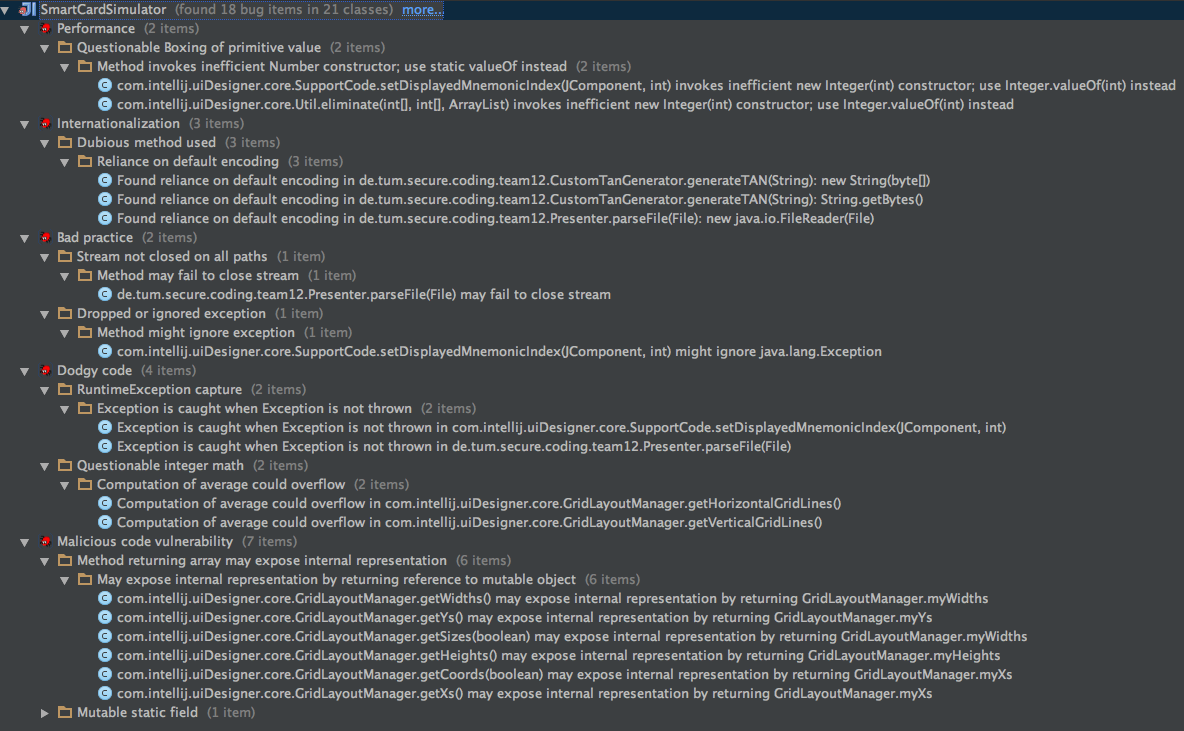
\includegraphics[width=\textwidth]{figures/gnb_findBugs}
	\caption{Analysis results for Goliath National Bank}
	\label{figure:gnb_findBugs}
\end{figure}

Not having found severe vulnerabilities through static code analysis, we did some further manual analysis on both applications.\newline
While analyzing the Bank System code we noticed that the application does not perform any user input validation, i.e. a user could insert arbitrary strings inside the PIN, destination and amount fields. This, however, does not pose any problems, as a TAN generated through invalid data will simply be rejected by the server.\newline
The GNB application, on the other hand, performs strict checks upon all user inputs, preventing any user from inserting invalid data. Pin, account number and transfer amount formats are already checked by the SCS application, discouraging the user from entering invalid data inside the web application at a later moment in time.

\clearpage
\subsection{TAN generation algorithm}
What follows is an analysis of the algorithm used by the Bank System application for generating TAN codes on the Java-based SCS application. This TAN then needs to be recognised by the web application without any interaction between the two.\newline
The algorithm can be found inside the \texttt{HashUtils.java} file and works as follows:
\begin{enumerate}
	\item Pin, destination account and amount to be transfered are concatenated inside a String in case of single transactions. In case of a batch transaction, the Pin and the whole content of the batch file are concatenated inside a String;
	\item A 5-digit nonce is randomly generated (i.e. an Integer between 10000 and 99999);
	\item The nonce is appended to the String obtained in the first step;
	\item The whole string is hashed using the SHA-256 function;
	\item The result of the hash operation (bytes) is converted into a BigInteger;
	\item The Hexadecimal String representation of the BigInteger is generated;
	\item As long as the length of the generated String is less than 64 characters, zeros are prepended;
	\item The first 10 characters of the String are taken and the previously generated nonce (5 characters) is appended;
	\item The resulting String has now a length of 15 characters and is returned to the user as the TAN.
\end{enumerate}
The generation of the 5-digit nonce provides randomness, hence two consecutives TANs will always look different, even though the input (i.e. PIN, account and amount) may be the same. The adopted solution also does not allow replay attacks: even though the nonce is random, making it theoretically possible to always use the same TAN for two identical transactions, this cannot happen since the server keeps track of the used TANs. This mechanism is visible inside the \texttt{/api/index.php} file (lines 130-140) and inside the \texttt{/api/asset.php} file (lines 511-524).\newline
Since the last 5 characters of each TAN, generated by the SCS, will always be numbers (i.e. the 5-digit nonce), it is easy for an attacker to guess the used algorithm. This however, doesn't prove the solution to be insecure, as a potential attacker can obtain the data inserted by the victim only by brute-forcing all possible combinations of Pin, account and amount. This is because the used function is a one-way hash function.\newline
This solution hence proves to be, in theory, secure against external attacks. Nonetheless, the application could incur into the following problems:
\begin{itemize}
	\item The random nonce could occur more than once for two identical transactions made by the same client. The resulting TAN would then be rejected by the server, since it has already been marked as used;
	\item Although very improbable, there could be hash collisions between two completely different transactions, leading to the same problem mentioned above (the nonce needs to be the same in this case as well);
\end{itemize}
The GNB Smart Card Simulator uses an approach that is very similar to the one we just analyzed for the Bank System application: the details of the transaction are hashed along with the Pin of the user and a 5 characters long timestamp (in base64). To avoid communicating with the server directly, the timestamp then replaces the last 5 characters of the resulting TAN, in order to allow the server to recompute the hash. Although it is harder to detect at first glimpse, since the timestamp has the same base64 format as the rest of the TAN, the used algorithm can still be guessed after careful observation. The principle, however, remains the same as the one previously described for the System Bank. The main difference is that no collision is possible in the GNB application, since strictly increasing timestamps are used instead of random nonces. Even in case of a hash collision, the resulting TAN would still be different than any other used before, hence unique.\newline
The GNB application presents a serious limitation though: since the timestamp used is only 5 characters long and is second-based (for better precision), the maximum timespan that can be covered in total is of 64\^5 seconds \= 34 years. This means that, in our case, the generated timestamps will overflow in approximately 22 years. After that date, the server will not accept further TANs anymore, since the timestamp will be lower than previously inserted ones. This bug is very similar to the year 2038 bug and should be fixed (i.e. handled differently) for long-term support.

\newpage
\section{C Parser}
\subsection{Reverse engineering}
By using the radare2 reverse engineering framework we obtained a disassembly of
all functions of the binary and a list of all symbols used in the binary.
Based on this information and with the visual support of the control flow graph
of the main function (see excerpt in \autoref{figure:re_cfg}) we created an
equivalent program included in the deliverables.

\begin{figure}[h!tbp]
	\centering
	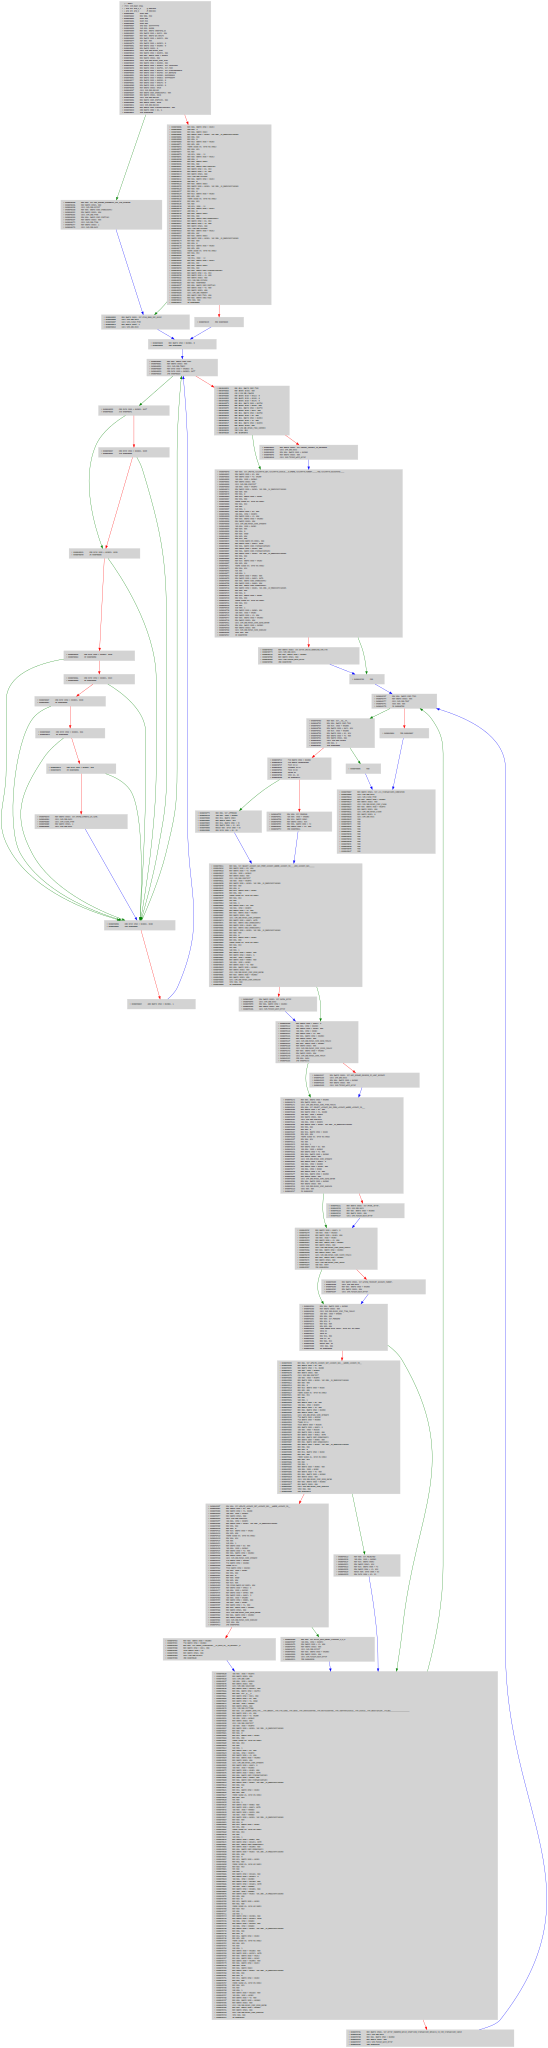
\includegraphics[trim={5cm 218cm 25cm 0},clip,height=\textheight]{figures/re_cfg}
	\caption{First part of control flow graph}
	\label{figure:re_cfg}
\end{figure}

\subsection{Extracted credentials}
As expected the C code contained the credentials required for a connection to
the database as it is required in order to perform the actual transactions.
\begin{itemize}
	\item \textbf{Database host} localhost
	\item \textbf{Database user} root
	\item \textbf{Database pass} crazypassword
	\item \textbf{Database name} Banking
\end{itemize}
No further credentials or hidden keys were discovered. The SQL statements used
in the binary can be viewed in the submitted reverse engineered c source code.

\subsection{Remarks on the C parser}
\subsubsection*{The whole program logic resides in the main function}
\begin{itemize}
	\item This leads to a single block of procedural instructions with
		over 750 lines of assembler code in the disassembly and over 250
		lines in the reverse engineered c code.
	\item Functions of this size make maintenance and testing harder
		and prohibit code reuse.
	\item The increased maintenance difficulty is visible on multiple
		occasions throughout the program. For example only 2 of 3
		malloced strings are freed on error, probably missed as it seems
		like the third string was added to a later date and the
		function size makes it harder to figure out all data
		dependencies.
	\item Separating the different parts of the program in individual
		functions with clearly defined interfaces is recommended.
\end{itemize}

\subsubsection*{Heap overflow}
\begin{itemize}
	\item The variables \texttt{sndaccount, inpfile and transactiontan}
		are initialized with a pointer to 200 bytes of allocated heap
		memory each. \newline
		\texttt{sndaccount = malloc(200);}
	\item This size limitation is not correctly enforced when copying data to
		these areas. The size of the data copied is only limited to the size of
		the string being copied instead of the size of the destination buffer.
	\item \texttt{strncpy(dst, src, strlen(src))} is used instead of \newline
		\texttt{strncpy(dst, src, 200)}
	\item This results in a heap overflow by specifying a parameter longer than
		200 chars to the script. The consequences of this overflow are
		documented in \vulnref{OTG-INPVAL-014-3}.
\end{itemize}

\subsubsection*{Error handling}
\begin{itemize}
	\item On multiple occasions return values are not checked for
		errors. For example none of the malloc calls check if the
		memory allocation was successful.
	\item The MySQL connection is not properly closed in case of error.
		Although this happens shortly before the end of the program,
		this might result in an increase amount of concurrent
		connections to the database before the connections are cleaned
		of automatically.
\end{itemize}
